\documentclass[aspectratio=169]{beamer}
\usetheme[block=fill]{metropolis}
\usepackage{tikz}
\usetikzlibrary{shapes.geometric, arrows.meta, positioning, calc}

\title{Building a Reproducible Scholarly Search Toolkit}
\subtitle{Episode 11: Response Normalization Subsystem}
\author{Scholar Search Kit}
\date{}

\begin{document}

\begin{frame}[plain]
  \titlepage
\end{frame}

\begin{frame}{Episode Goal}
  \begin{alertblock}{The Goal}
    Create a flexible parsing toolkit to safely map chaotic JSON into our clean \texttt{Document} and \texttt{Author} models.
  \end{alertblock}
  \vspace{0.5cm}
  We established the \texttt{Document} model in Episode 4. Now we build the factory tools that will populate it without crashing when fields are missing or misformatted.
\end{frame}

\begin{frame}{The Normalization Philosophy}
  \begin{block}{Defensive Extraction}
    Never assume a JSON field exists or is the correct type.
  \end{block}
  
  \begin{itemize}
      \item \texttt{FieldExtractor}: Safely fetches deeply nested keys (e.g., \texttt{metadata.authors[0].name}).
      \item \texttt{DateParser}: Converts "2023", "2023-05", and "2023-05-12" to clean integers.
      \item \texttt{IDExtractor}: Leverages the regex logic from Episode 3 to populate \texttt{ExternalIds}.
  \end{itemize}
\end{frame}

\begin{frame}{Implementation: `ResponseNormalizer` Protocol}
  \begin{center}
  \resizebox{0.65\linewidth}{!}{
  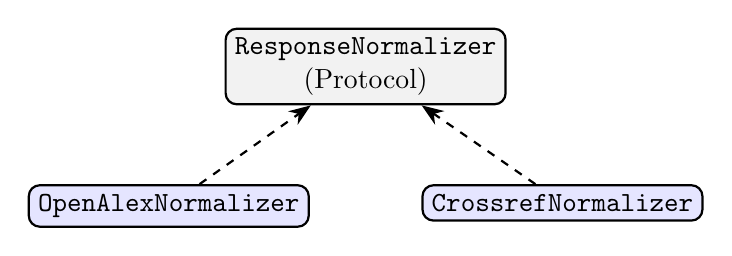
\begin{tikzpicture}[
      node distance=1.5cm and 2cm,
      base/.style={rectangle, draw, thick, rounded corners, minimum width=3cm, align=center, fill=black!5},
      impl/.style={rectangle, draw, thick, rounded corners, minimum width=3.5cm, align=center, fill=blue!10},
      arrow/.style={-{Stealth[scale=1.2]}, thick, dashed}
    ]
    
    \node[base] (proto) {\texttt{ResponseNormalizer}\\(Protocol)};
    
    \node[impl, below=1cm of proto, xshift=-2.5cm] (oa) {\texttt{OpenAlexNormalizer}};
    \node[impl, below=1cm of proto, xshift=2.5cm] (cr) {\texttt{CrossrefNormalizer}};
    
    \draw[arrow] (oa) -- (proto);
    \draw[arrow] (cr) -- (proto);
  \end{tikzpicture}
  }
  \end{center}
  \vspace{0.5cm}
  Every Provider implements this interface. It exposes a single \texttt{parse(raw\_data)} method that guarantees a \texttt{Document} out.
\end{frame}

\begin{frame}{Verification}
  \begin{alertblock}{Success Criteria}
    \begin{itemize}
        \item Fetching a missing key returns \texttt{None} instead of throwing \texttt{KeyError}.
        \item Date parsers correctly fallback to \texttt{None} if the string is garbage.
    \end{itemize}
  \end{alertblock}
\end{frame}

\end{document}
